\documentclass[]{report}
\usepackage[style=authoryear]{biblatex}
\addbibresource{references.tex}
\usepackage[utf8]{inputenc}
\usepackage[T1]{fontenc}
\usepackage{graphicx}
\usepackage{subcaption}
\usepackage{hyperref}
\graphicspath{images}

\hypersetup{
	colorlinks=true,
	linkcolor=blue,
	filecolor=magenta,      
	urlcolor=cyan,
}

\urlstyle{same}

% Title Page
\title{NES Emulator}
\author{Sebestyén Bence}

\begin{document}
\maketitle

\tableofcontents

\clearpage

\chapter{Introduction}

\paragraph{}
The Nintendo Entertainment System, frequently called NES, is an home gaming console developed by the Japanese company called Nintendo Company, Limited.  Through it's lifetime the from the earl '80s up until the end of the '90s a lot of good quality titles were released to the platform and a wide range of audience were reached. Due to this quality of games and  popularity which the NES gained at it's peak time people even nowadays like to pick up some of the most famous, or personal favourite titles and play through them. Sadly, due to the rapid evolution computing the current hardware are not compatible with the old games developed for the NES platform also the old and still working consoles are really hard to get a hands on. Yet the gaming community still keeps alive these games and the way it is mostly done by using emulators.

\paragraph{ }
To solve the compatibility issue with the modern hardware, without actually buying or refurbishing one, the community started to creating so called emulators. Which are a special kind of software, it's purpose is to provide a virtual emulator environment of a given old or very specific hardware, such as the NES for instance, on top of a given system, like PC or any other gaming console. This projects goal is to produce an emulator like this which, by emulating the NES hardware behaviour, provides a way to run the games without any need of the modification of the old games code. Therefore, unlike porting the actual game, the user has access to an authentic experience. On the other hand, emulation is more resource dependent than a ported game, but less time consuming than porting every single game.

\section{History}

\paragraph{ }
 This console was the second console of which was created by the Nitnedo Co. Ltd. and the first which was planned to be sold worldwide (\cite{HIST}).
The gaming console was first released in Japan in 1983. The Japanese version was called Famicon and had a bright red toy-like design, unlike the version which was released worldwide.
The homeland release was followed by the USA and parts of Europe in 1986 and later in 1987 Australia and the rest of Europe.
\paragraph{ }
However, these releases were concerning for Nintendo as '83 was also the year of the great video game crash happened in North America (\cite{CRSH}). But it turned out the perfect opportunity for the console. As the hugely saturated gaming console market shrunk down, most of the competitors get bankrupt, Nintendo rebranded their console and released it as Nintendo Entertainment System worldwide.
\paragraph{ }
 It was a huge success not just because the competitors fall out but also due to two important principle which Nintendo following since then. One of them is unlike other consoles before only certified games could be released to the platform, which meant degradation in quantity and increase in the quality of the games. The other principle was that the actual hardware built from not bleeding edge components therefore making it cheap, more easily accessible.
 
\begin{figure}[!htb]
	\centering
	\begin{subfigure}[b]{0.4\textwidth}
		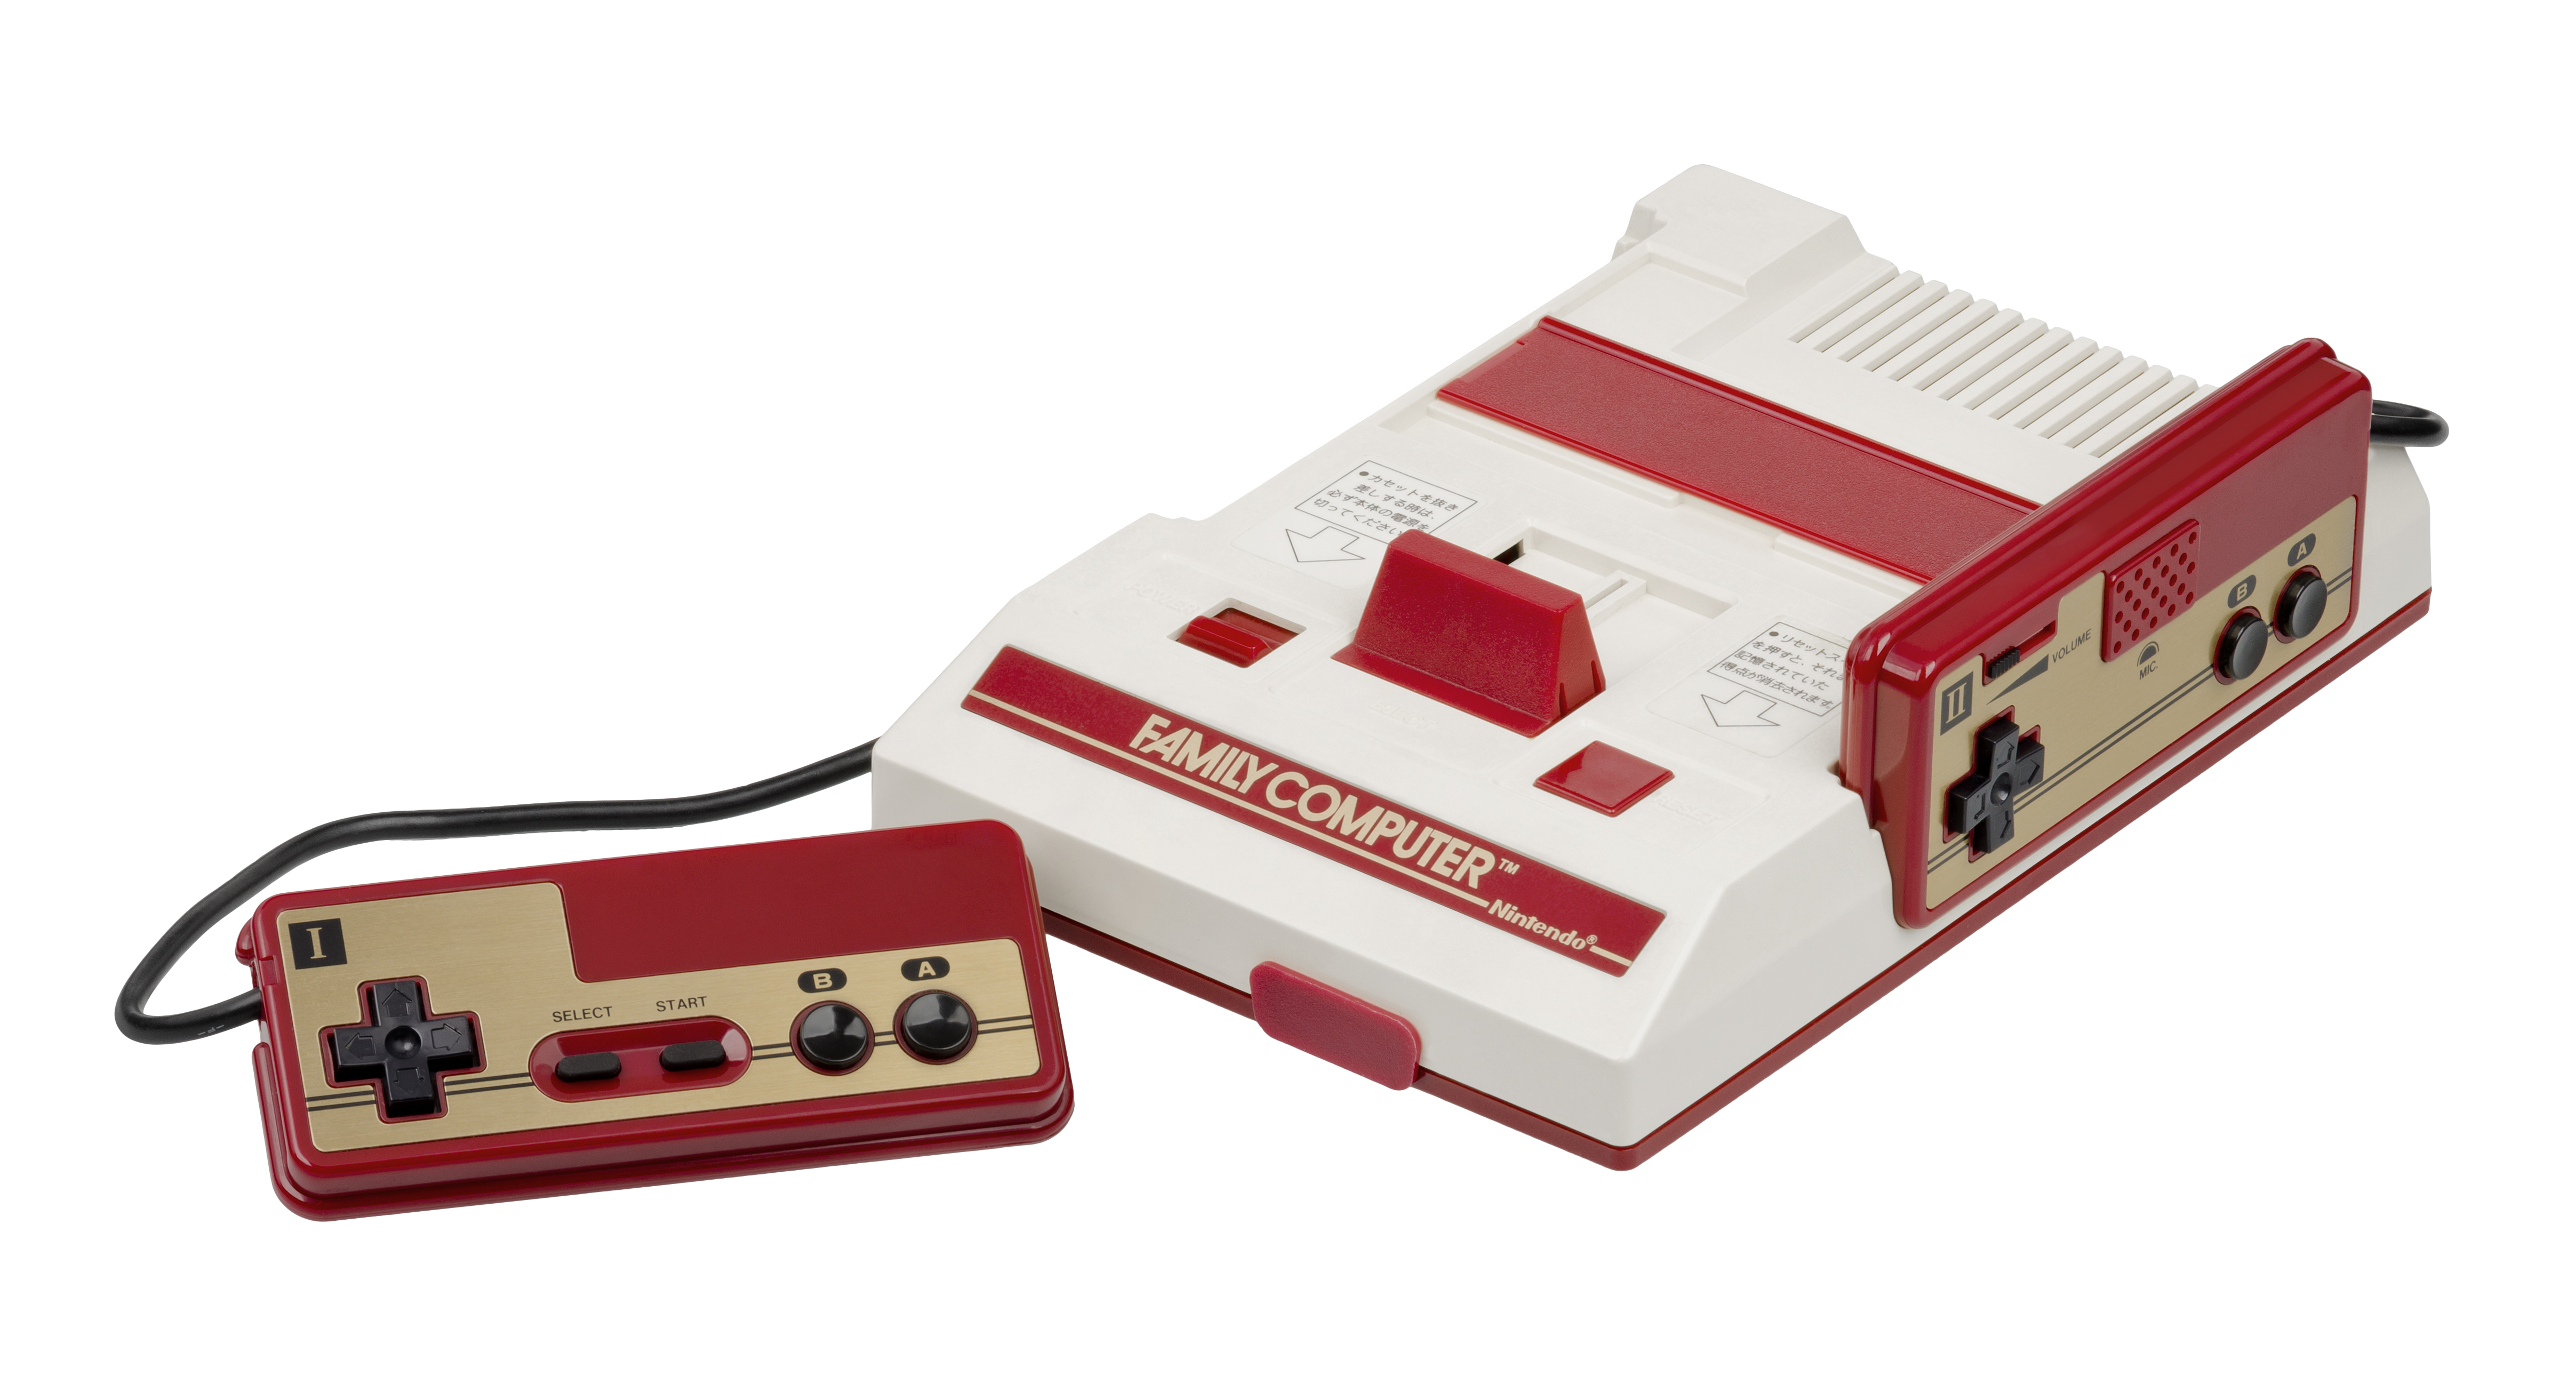
\includegraphics[width=\textwidth]{images/famicon.jpg}
		\caption{Famicon}
		\label{fig:1}
	\end{subfigure}
	%
	\begin{subfigure}[b]{0.4\textwidth}
		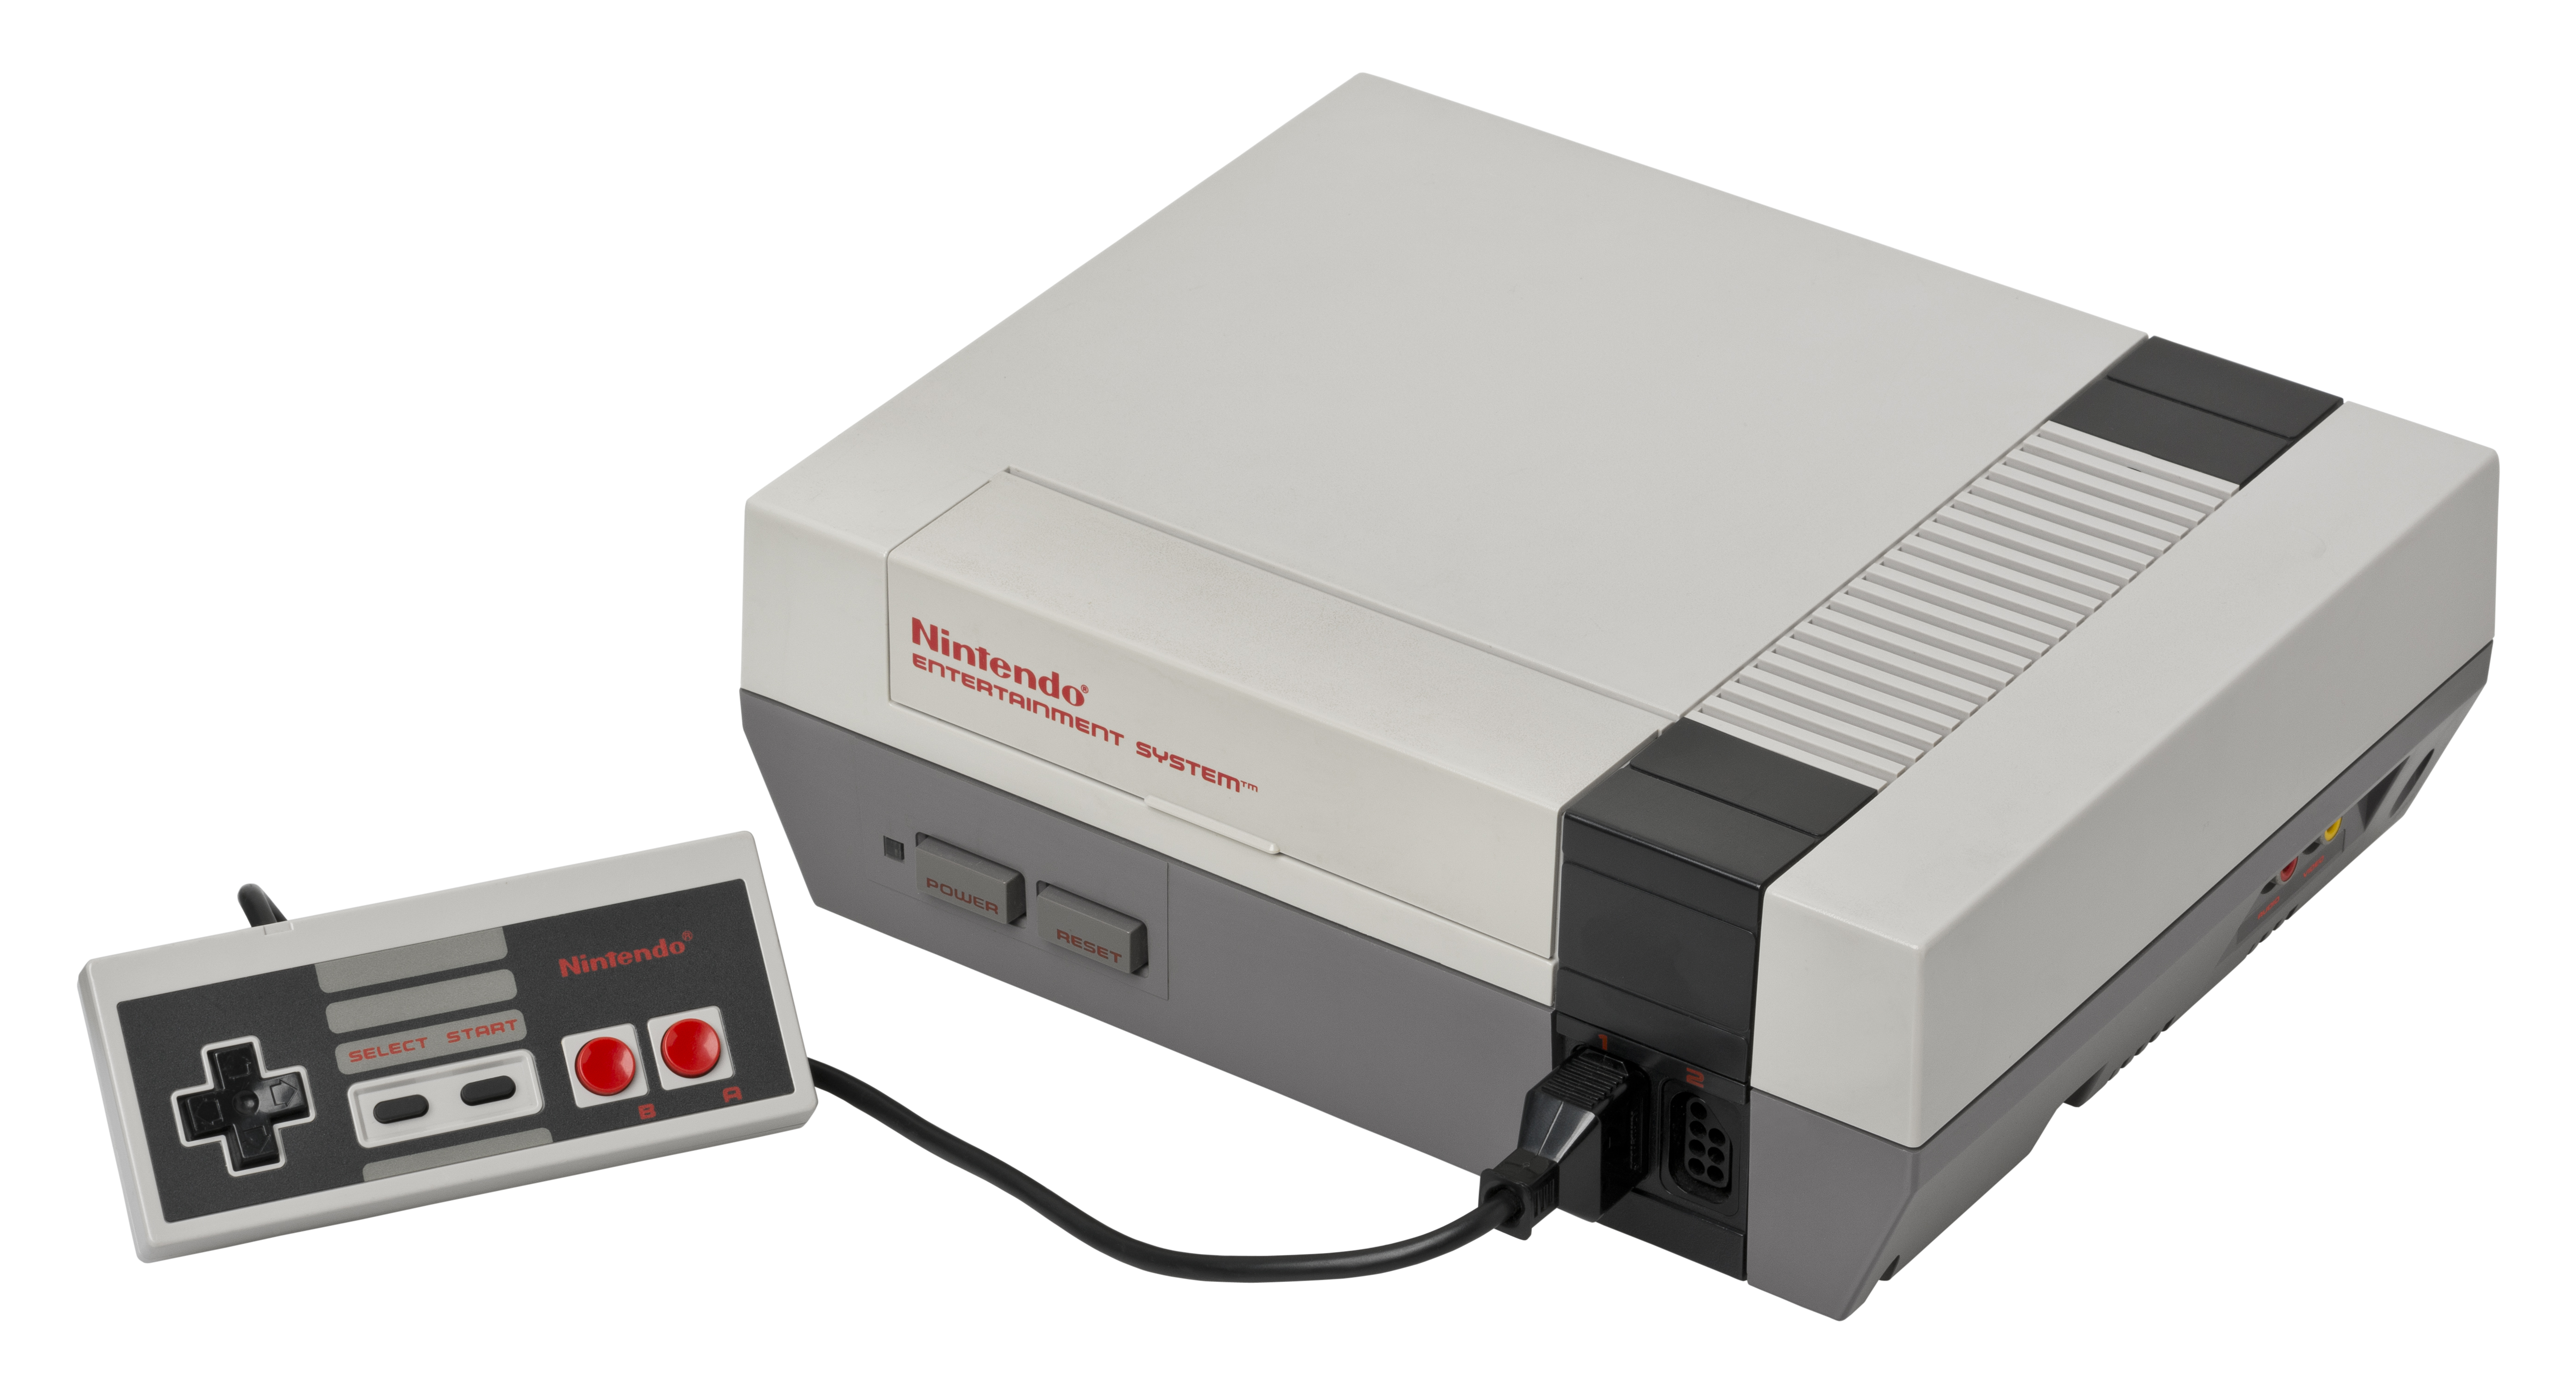
\includegraphics[width=\textwidth]{images/nes.jpg}
		\caption{NES}
		\label{fig:2}
	\end{subfigure}
	\caption{\label{fig:my-label} The console design}
\end{figure}
\clearpage



\section{Background}
\paragraph{ }
The NES hardware itself can be divided up to five big different part. 
\paragraph{ }
The console main chip was manufactured by Richo, which contains the CPU (Central Processing Unit) and the APU (Audio Processing Unit) (\cite{CPU}).  
The processor itself is an 8-bit MOS Technology 6502 with a little difference that the decimal mode is not presented. 
\paragraph{ }
The PPU (Pixel Processing Unit), which was also shipped by Richo, is technically a primitive graphics card which is used by the system to colour and render the graphics pixel by pixel to the Television screens.
\paragraph{ }
The Cartrdige which meant to provide the necessary binary code of the games and also the graphics data for the system. Also gave an opportunity to the developers to implement their own cartridge builds and use it to extend the console's capabilities one great example for that is the first The Legend of Zelda game. The game's cartridge also contains a battery powered RAM extension for players to save their game state (\cite{ZELD}).
\paragraph{ }
Two 8 button, these buttons are up, down, left, right, select, start, A, B, controller provided the interface for user input to the system. The NES controller was the first controller which introduced the single button plus symbol shaped DPAD. Each Nintendo system was brought some revolutionary design idea to the world of gaming console controllers.
\paragraph{ }
The RAM (Random Access Memory) is the central piece of the hardware which not only holds data but trough memory mapping it also connects all the other pieces to the CPU. Therefore the developers can control the full hardware behaviours trough with specific read and write operations to certain memory slots.
\paragraph{ }
In this project, these core parts of the hardware will be emulated on x86-64 machines. As a result, provide an application which is able to run those games which were developed for the original NES system.

\begin{figure}[!htb]
	\center{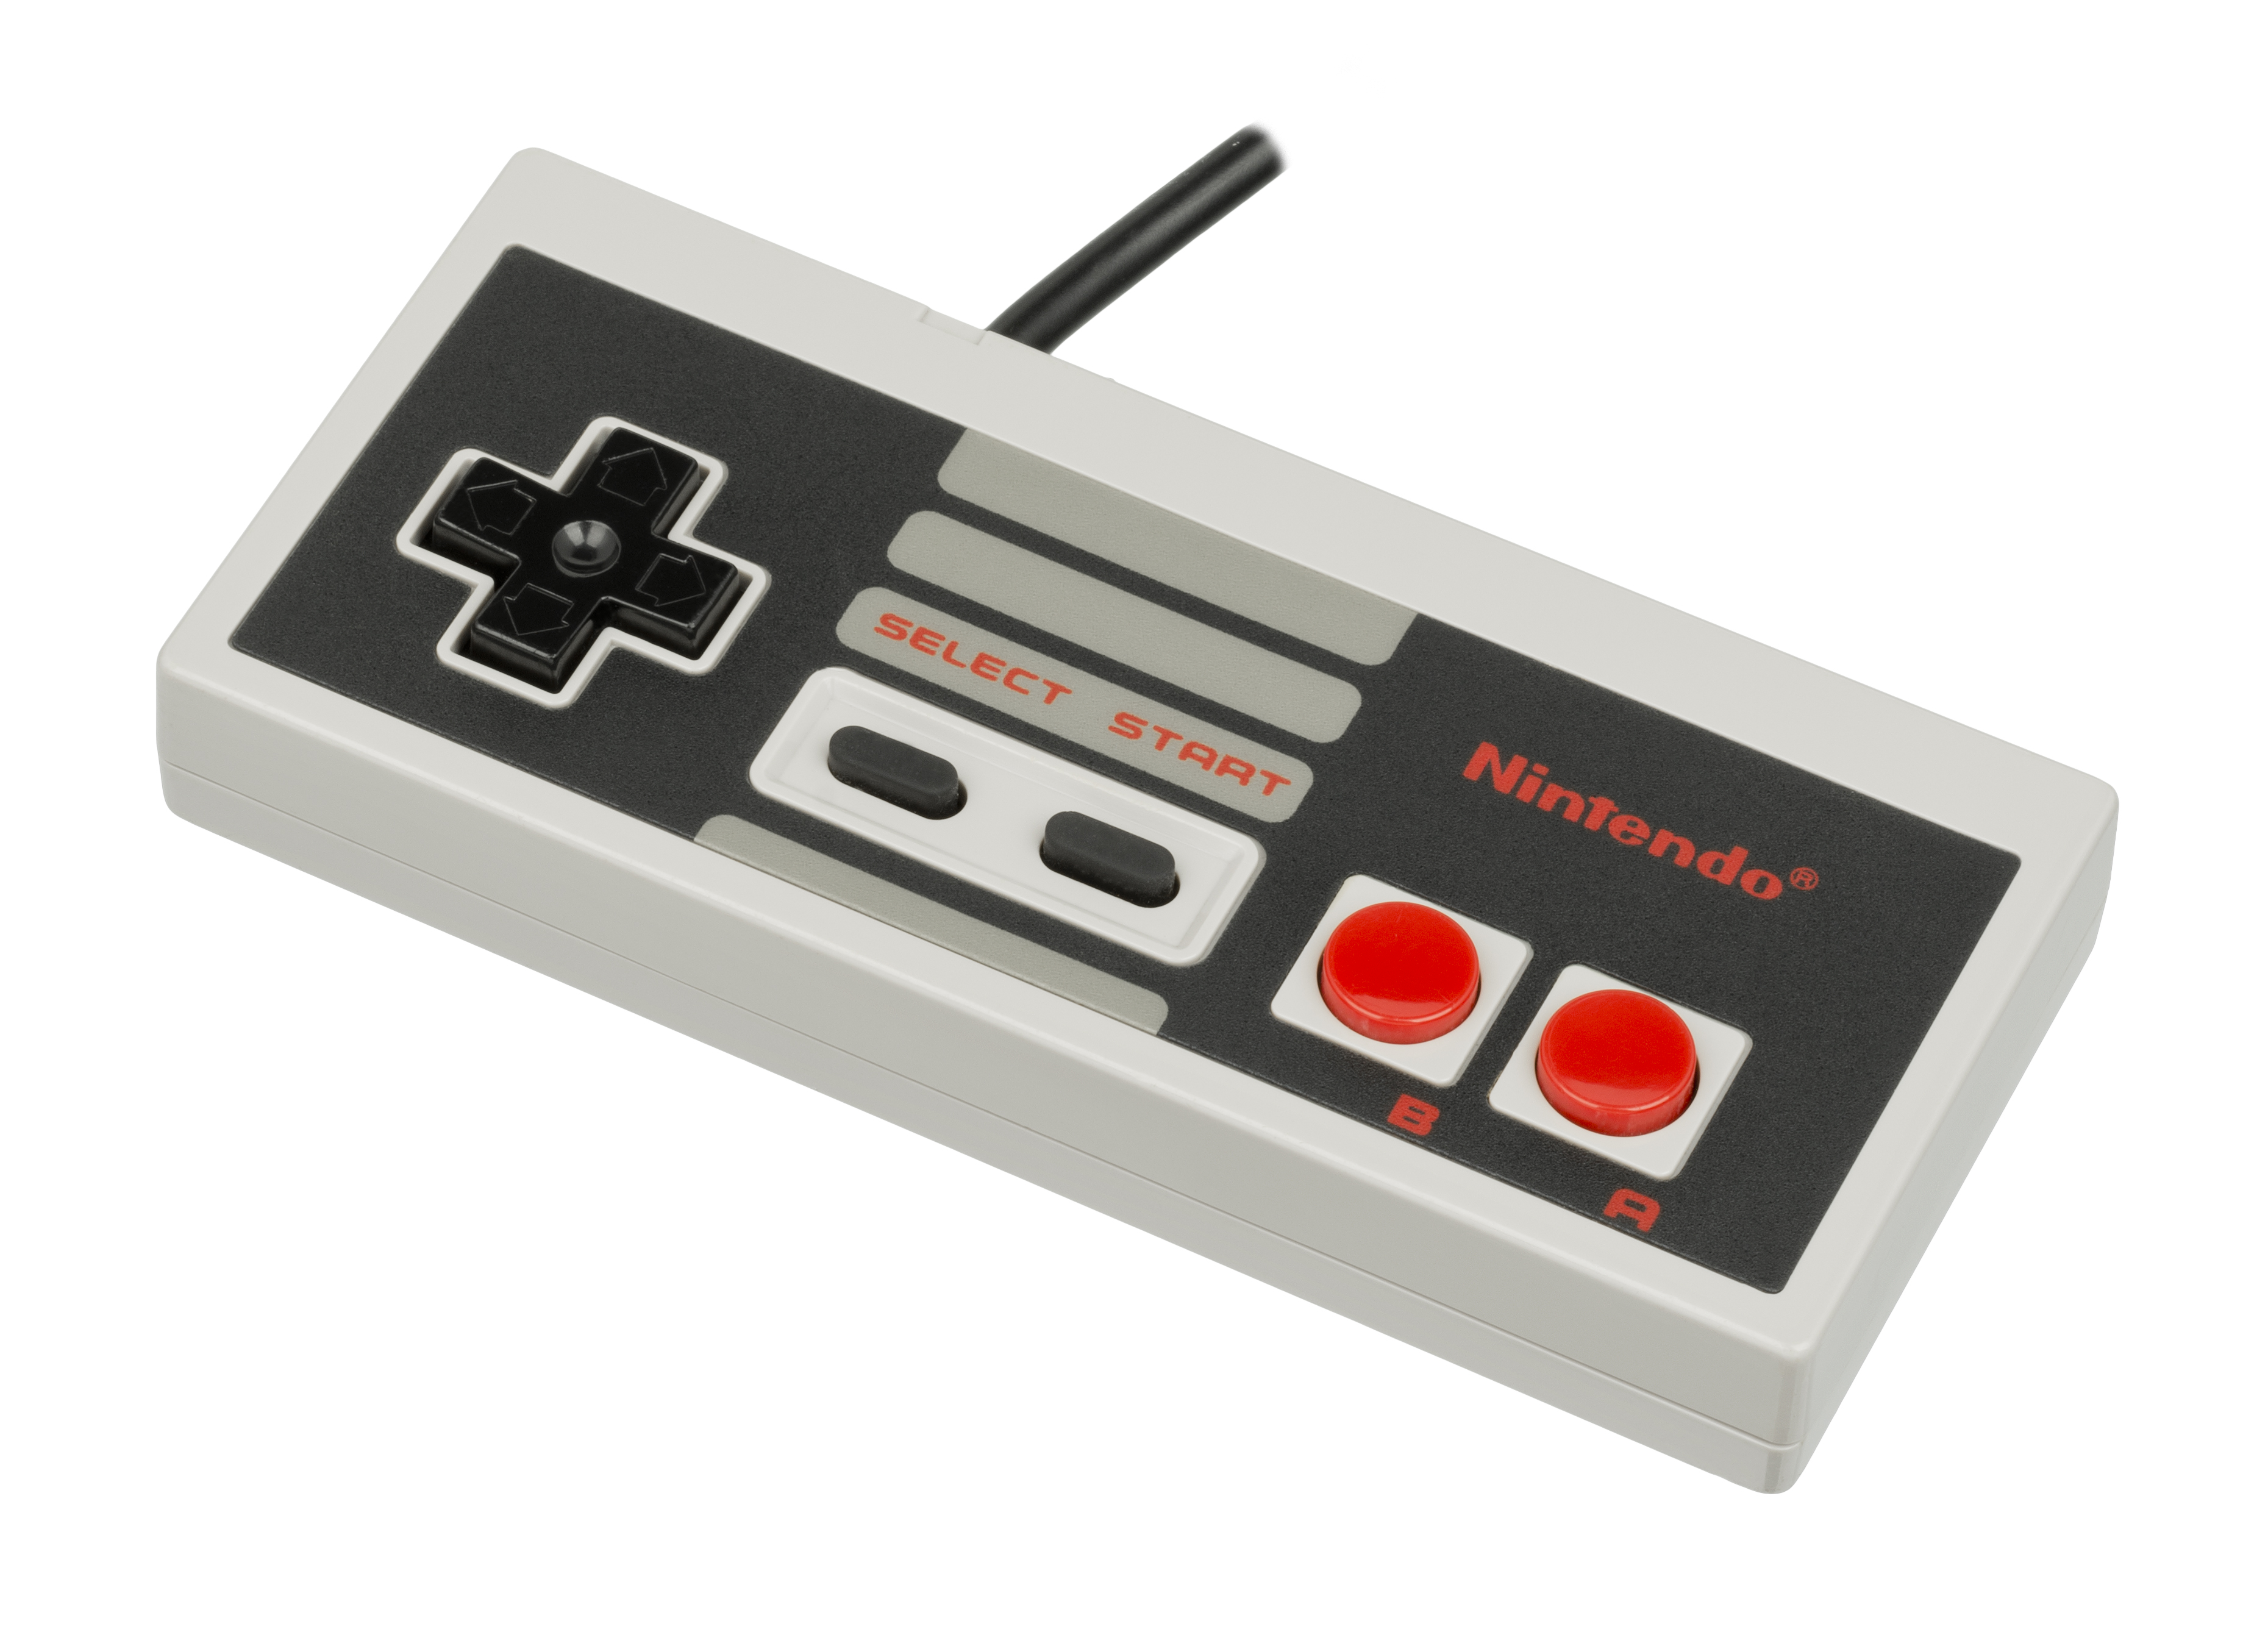
\includegraphics[width=\textwidth]
		{images/nes-controller.jpg}}
	\caption{\label{fig:my-label} NES controller}
\end{figure}
\clearpage



\chapter{Project Goal}
\paragraph{ }
The main target of the project is to build an application which is able to run games developed for the original Nintendo Entertainment System. The main target platform for the emulator to support is 64bit Linux, but the project design allows easy implementation for other platforms too. This goal is achieved by emulating all the necessary hardware of the original NES system programmatically thus creating a medium for the game binaries to run without any modification at all to it. 
\\ 
However, as the sounds system (APU) is not necessary to be able to run the games this part of the system is not implemented.
\\
The project goal can be divided into multiple stages which are the core and other advanced stages.
The main goal is to achieve the Minimal Core stage by the project deadline. However, if the time allows it advanced features will be implemented. 
\paragraph{Core - Minimal}
The emulator can emulate the perfectly the RAM and it's mirroring mapping behaviour properly. 
\\
The CPU capable to execute all the official operation codes, as the MOS 6502 has unofficial operation codes as well, also able to properly handle interrupts. 
\\ 
Graphics displayed on the screen with the usage of the PPU without any restriction about how it is doing it.
\\ 
The user is capable to interact with the system with a keyboard.
\\ 
Digitalized cartridge format (iNes) red and mapped with the basic NROM mapper (Mapper 0).
\paragraph{Core - Full)}
The graphics CPU and the whole system itself running with 100\% cycle accuracy compared to the original gaming console.
Some games are heavily rely on cycle accuracy, especially to provide some nice graphics implementations and also to provide more authentic experience for end users.

\paragraph{Advanced - Mappers}
Implementing additional Cartridge mappers other than the basic NROM mapper\cite{MPPR}. This would allow the emulator to run a larger pool of games.

\paragraph{Advanced - Multiple Platform}
Due to the nature of the project design, see below, support for other systems could be more easily implemented due to the modular approach which was used to develop the emulator. Therefore for instance Windows and Android could be easily supported by the emulator which would further boost the user experience.

\paragraph{Advanced - State Save}
Allowing the user to make a snapshot of the current CPU PPU and RAM state and be able to load it back at later point in case if the user would like to continue the game right from the place where they saved it.

\paragraph{Advanced - Online Multiplayer}
The NES system supports two-player local multiplayer, as the system provides hardware to connect two controllers, by default which could be extended over a network, therefore, players could play two player games with the comfort of their homes.

\chapter{Project Execution}

\section{Design}

\paragraph{ }
Due to the fact that the NES gaming console's hardware could easily be divided up to 6 distinct, loosely coupled module, it was clear that the best way is to design the implementation around these modules:
\begin{enumerate}
	\item Ram
	\item CPU
	\item PPU
	\item Controller
	\item Cartridge / Mapper
	\item APU
\end{enumerate}

This thanks to the fact that the system gives control over all of these pieces by wiring them into given memory slots and using CPU instructions to perform read and write instructions on them to trigger given actions on them, all of this without letting the actual CPU Hardware know that it is accessing anything else. Therefore when the system could be implemented module by module in careful order. Due to this modular separations, it was easy and straightforward to build each module easily by separating them up to smaller task and gradually build each module.
\paragraph{ }
Besides the separation of the emulator code to modules, the GUI, Graphical User Interface,  is also separated from the actual emulator logic. This behaviour is implemented by compiling the NES emulator logic into a shared object, dynamic library for Windows users, and linked it with the GUI implementation. This decoupling has numerous advantages over shipping the whole application as a single executable.
\\ 
Due to this separation, the emulator logic became easier to test on its own. 
\\ 
When a new patch is ready for the applications only part of the project needs to be recompiled and updated. Which makes easier to implement a versioning and updating system.
\\ 
The GUI implementation can be changed without affecting any of the core solutions therefore it is easier to port it to different platforms and devices.

\section{Tools}
\paragraph{ }
The project is written in the latest standard of C++ 17 (\cite{CPPV}). The reason behind the choice of C++ was that the language itself really stable and mature and proven to be a great tool to develop clean, stable, high performant software solutions and also providing low-level solutions for given sets of problems such as pointers. Compared to C, a system level programming language, C++ provides a more readable code on exchange for minimal performance loss thanks to it's rich standard library and object oriented programming capabilities.

\paragraph{ }
On the top of C++ a small number, namely two, of external libraries were used to develop the project.
Catch2 (\cite{CTCH}) was used to carry out the automated tests which were written for the project in a BDD (\cite{BDDT}) style.
The other one is SDL (\cite{SDL2})

\paragraph{ }
For source code compiling the GCC (\cite{GCCV}) version 8.2.1 toolchain is used through the MAKE (\cite{MAKE}) build system. And these are configured with CMake (\cite{CMKE}) to which provides a cross-platform build tool configuring interface. Also, it provides an opportunity for developers to use their own preferred IDE, Integrated Development Environment, therefore boost their productivity.

\paragraph{ }
The project documentation consists of two parts the report itself (this document) and the API doc (\cite{APID}).
\\
The report was created with LaTeX (\cite{LATX}). On the other hand, the API documentation was generated with Doxygen (\cite{DOXY}) from the annotated C++ Header files of the source code.

\paragraph{ }
The source code along with the build system configuration and the documentation is version controlled with GIT and stored in a main  Github repository (\cite{REPO}).
As the project meant to be published as an open source project it is publicly available. Although, under the time of the project during the course of the project it was also publicly available the repository was strictly available for editing for the project owner (Sebestyén Bence) and the project supervisor (Robert Atkey).
\\
The project repository is also linked to a CI, Continuous Integration, the system called Travis CI (\cite{TRAV}). Which mostly used to provide security against merging any proposed changes which are not passing the build state or failing any of the automated tests which were supplied with the source code. The CI system build and testing are triggered every time when a pull request for a change against the main repository is set up and blocking any merge until the errors within the proposed changes are not fixed.



\section{Management}

\paragraph{ }
The development cycle managed through GitHub project page. For every task regarding the project execution, there was an issue opened. These issues were labelled up based on which development cycle, see below, it was accomplished, and added to the given project milestone based on which module it was belonged to.
\\
This provided a great oversight over the project's evolution and also a faster more stable development cycle due to the small subtasks.

\paragraph{ }
The development life cycle contains multiple stages which are built upon each other. These life cycle stages are the following:

\begin{enumerate}
	\item Planing
	\item Prototyping
	\item Implementing
	\item Testing
	\item Documenting
\end{enumerate}

\paragraph{ }
Every small task went through a planning phase which mostly consisted idea how to actually code down the given task and how it is going to be fitting into the whole project current state meanwhile thinking about to keep as much space as possible for later new features and improvements.

\paragraph{ }
Prototyping itself was more flexible, compared to the planning, it was different from task to task, some sort of prototype was also developed outside the project source to prove concepts of the planning, but the difference was that it was not always done to every single subtask. Sometimes it involved a whole module, sometimes it just has done for two tasks together.
\\
The main goal here was to test the result of the planning in an actual working context and see if the result is clean, stable and extendable enough to be implemented in the actual project.

\paragraph{ }
Through the implementation, the actual result of the planning and prototyping were added to the main code base.

\paragraph{ }
Testing was carried out in two phases. Depending on the given issue, manual testing was carried out on task and a subtask level if it was needed and also automated BDT, Behaviour Driven Testing, where implemented for every module to test their provided functionality. And these automated tests were executed with the CI as well.
%
\paragraph{ }
The API documentation were created after the given task was finished and updated with Doxygen.
\\
Meanwhile, the report itself was uprated in larger chunks because this way there was always a bigger portion of the system was available therefore it was easier to position the actual chunk to the whole project.

\begin{figure}[!htb]
\center{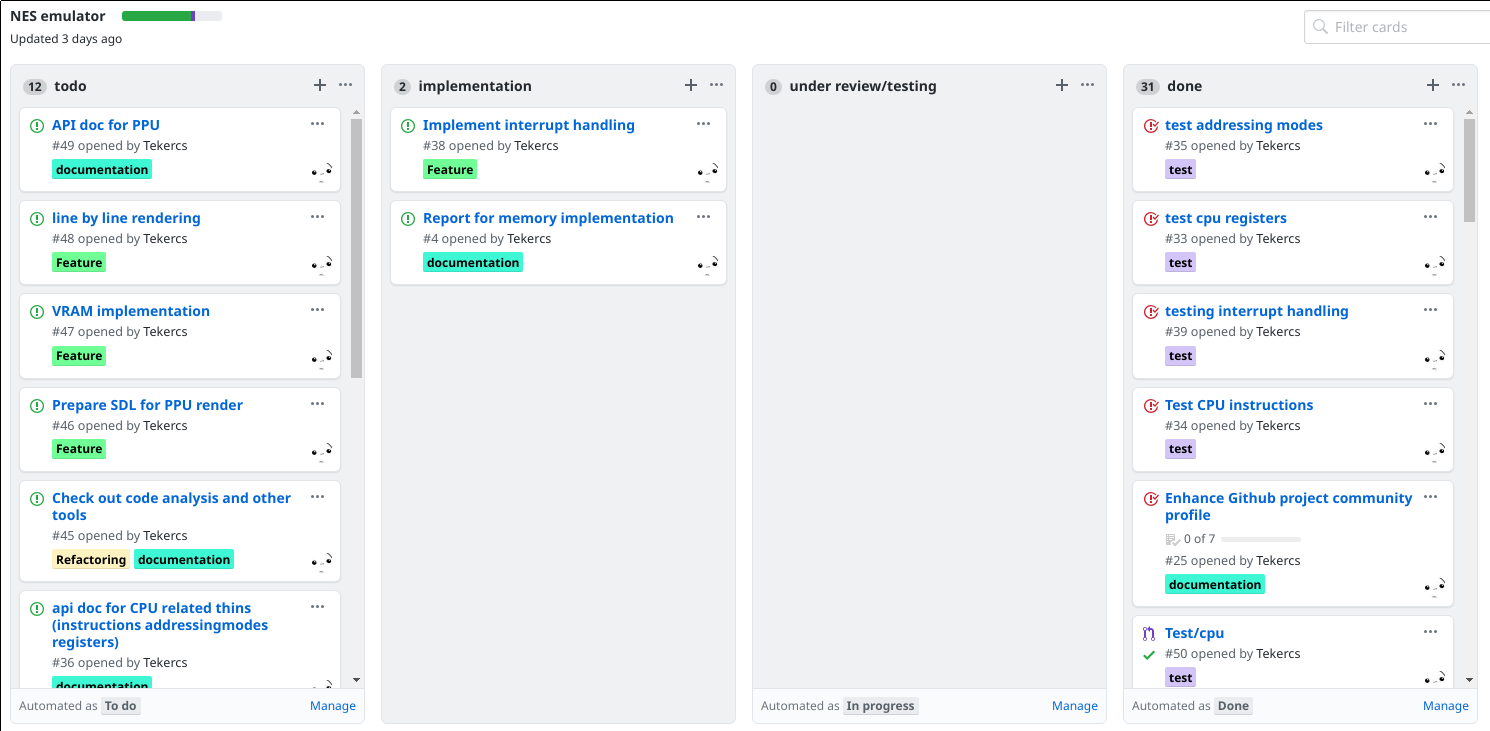
\includegraphics[width=\textwidth]
	{images/github_project.png}}
\caption{\label{fig:my-label} Github project page}
\end{figure}
\clearpage

\chapter{Specification and implementation}

\section{CPU}

\subsection{Specification}

\paragraph{ }
The NES CPU was the RP2A03/RP2A07 chip, a modified version of the MOS 6502 (\cite{6502}) microprocessor, manufactured by Ricoh (\cite{RCHO}). This chip was an 8-bit little-endian microprocessor running on 1,79/1,66 MHz, the European / Australian version (PAL) was running on a lover clock speed.
\\
The CPU contains 6 registers from that 3 are more general purpose  and 3 are special purpose (\cite{REGS}).
\begin{enumerate}
	\item Accumulator
	\item X index
	\item Y index
	\item Status flags
	\item Stack  pointer
	\item Program counter
\end{enumerate}

All of these registers are 8-bit long registers except the Program counter which is 16-bit long due to the memory address bus size, see below (\cite{REG2}). Most of the work was done on the Accumulator, X and Y index registers
as the most of the arithmetic and load/store instructions were implemented for these. Also the result of these operations were visible on the Status flags as well. 
\\
The Status flags was an 8-bit register where each bit, except the 5th bit, are representing a different state of the CPU. 
\paragraph{Negative Flag, 7th bit}
This flag is changed whenever the last CPU instruction's result is negative or not. The reason why this flag is important is the CPU's instructions on its own can not determine if the given 8-bit value which it is working with at the moment is negative or positive. Therefore this flag is used to tell the programmer about the result and give the control to their hand to handle the result in way as it is good for them. By ignoring the flag the result can be treated as an 8-bit long unsigned value or, with the value of the flag kept in mind, as an signed 8-bit value.
\paragraph{Overflow flag, 6th bit}
The value of this flag determined by the sign flag of the result of the previously executed instruction is invalid or not.

\paragraph{Break flag, 4th bit}
Whenever the programmer decides that they want to force out an interrupt from the CPU by executing the BRK, Break, command this flag is set. Therefore the CPU know that after finishing the instruction an IRQ interrupt should be handled.

\paragraph{Decimal Mode, 3rd bit}
Decimal mode flag can be toggled by two CPU instruction, but has no effect on the system due to the fact that the custom modified chip which is used by the emulator is not implementing this binary-coded decimal mode.

\paragraph{Interrupt Disable, 2nd bit}
This flag also connected to the chips interrupt handling. As if this flag is set, then the microprocessor will ignore al the IRQs. 

\paragraph{Zero Flag, 1st bit}
Whenever an arithmetic operation's result are zero this flag is set. It is important not just for arithmetic but control-flow instructions using it as well for their checks whenever the processor should branch or not.

\paragraph{Carry flag, 0th bit}
The flag is set by either its designed instruction, or any other arithmetic, shifting or rotating instruction which result did not fin in the 8-bit size.
This is important to provide support for operations on larger values than 8-bit. One of the reasons is the fact that the memory's address bus is 16-bit. 

\paragraph{ }
Along the register the other main capability defining aspect of the chip is it's instruction set. Due to its 8-bit nature of the microprocessor the number of available instructions are 256. Although not every opcode is implemented officially (\cite{INST}). The 151 instruction which actually implemented are technically 56 instructions with different addressing modes (\cite{ADDR}). Each instructions has its execution time measured in CPU cycles, which depends on the addressing mode and the length of the instruction itself. Usually the instruction are a 1 - 3 byte long, the 1st byte specifies the instruction and it's addressing mode and the optimal 2nd and 3rd are used to specify the operands of the instruction. For example:
\\
\\
TXA instruction is 1 byte long.
\\
STY \$01 is 2 byte long 
\\
STY \$20AA is 3 byte long
\\
\\
Important to notice that the Indirect jump instruction, JMP (opcode: \$6C), contains a bug. When ever the indirect instruction parameter points to \$xxFF, where x is any hexadecimal number, the instruction fetches the low-byte from \$xxFF then the high-byte from \$xx00 instead of \$(xx+1)00. This is an important bug because there are games which heavily rely on the the behaviour of this instruction.

\paragraph{ }
As it seen above on the STY example the same instruction could behave differently this is due to the different addressing mode. Each instruction has its own set of addressing modes,  these are all the possible ones: 

\begin{enumerate}
	\item Implicit
	\item Accumulator
	\item Immediate
	\item Zero Page
	\item Zero Page,X
	\item Zero Page,Y
	\item Relative
	\item Absolute
	\item Absolute,X
	\item Absolute,Y
	\item Indirect
	\item Indexed Indirect
	\item Indirect Indexed
\end{enumerate}

\iffalse
maybe describe each addressing mode
\fi

\subsection{Implementation}
When it came to implement the processor emulation it was carried out in multiple stages.
\paragraph{Registers}
First of all the register emulation had to be implemented first, as all of the CPU instructions accessing at least one of the registers. Each of the registers is emulated by a \textbf{\textit{uint8\_t}} typed variable, or  \textbf{\textit{uint16\_t}} for the program counter, wrapped in a class called  \textbf{\textit{Registers}} (\cite{DREG}) with the necessary accessors functions implemented within. This separation from the actual CPU logic is the result of the break up of the big classes for testing and readability purposes.

\paragraph{Instructions and Addressing modes}
The first thing to start with instruction implementation is to separate the logic of the addressing mode and the core instruction itself.
\\
 For instance, the ADC instruction has 8 different addressing mode. Each of them specifies the way how the instruction obtains the 8 bit value which then will be then just added to the accumulator along with the carry. 
 With this separation there were only need for 51 core instruction implementation and separately 13 addressing mode instead of the total 151 instruction. 
\\
Each of the instruction and addressing mode implementation received it's own function (\cite{DCPU}) to make the code as easy to read/understand and debug as it is possible.

\paragraph{Memory accessing}
As some of the instructions are accessing the main memory of the system for either reading or writing. Therefore  the  \textbf{\textit{Cpu}} class also receives a smart pointer to a \textbf{\textit{Memory}} object, for implementation details see below.

\paragraph{CPU Cycle}
The CPU Cycle emulation was implemented with a different approach. As there is no straight correlation between the cycle and anything else, other than the fact that the PPU itself roughly working on 3X as much cycle rate, the possibility is open to implement it to check for interrupts and  execute a single instruction in each step instead of just a single cycle (an instruction usually executed through several CPU cycles 2 - 7 cycle/instruction). 
\\
Due to the computational power difference between the NES and the today's average PC this approach does not prevent emulator to work with 100\% cycle accuracy. As even the most complex instruction can be easily executed within the necessary time frame even with the fact that the emulator running on the top of the normal system. This of course could cause issues within an emulator if the emulator's target platform would be stronger such as an Xbox 360, PS 4 or Nintendo Wii.
\\
The instruction execution implementation is consist of a mapping of the 8-bit opcode of the instruction to a paired function call for the core implementation and the addressing mode. This mapping is implemented with a switch statement which readability wise is not the best option due to it has 151 case but that is nearly the best way performance wise.
\\
Although, if it is needed there is room for further performance increase. By monitoring the emulator through different games it is possible to find the most used instructions. With this information in hand, the most used instructions could be lifted out from the switch statement and implemented with an if-elseif structure, in order the most used ones checked first and the least used one checked last from the selected set of instructions. By doing that, the compiler could actually provide further optimization on this part of the implementation.


\subsection{Testing}
\paragraph{ }
The testing of the CPU was carried out by using a test cartridge developed by Kevin Horton (\cite{NEST}). As his test ROM is an all inclusive test when it comes for CPU and its instruction's behaviour.
\\
The test carried out by implementing a helper logging function for the CPU implementation. A state log was generated based on the upcoming instruction to be executed and the current state of the registers. Then this log was compared in every processor cycle with a log which was provided along with the test ROM. 
As the invalid opcodes was no implemented in the project those tests were skipped.
\\
Testing these type of software happens to be challenging. Even the fact that a pre-written testing ROM were used] to identify if any bug left in the system, finding the actual source of the problem was proved to be challenging. Mostly to follow trough instruction by instruction the executed operations to see which instruction's resulted faulty execution. Besides it is time-consuming and requires the tester to maintain the track of the execution in real time with the software as the problem source from time to time can even happening in a completely different execution step compared to where the bug were actually found.
\\
The most effective bug findings were the result of using a debugger tool and next to it a pen and paper approach.
\paragraph{ }
Also along the implementation phase when it came to implement the instructions and the addressing modes.
Each of them after implementation were tested manually as well. Due to the fact that the testing ROM mentioned above was only usable after the whole CPU emulation completed.

\begin{figure}[h]
	\center{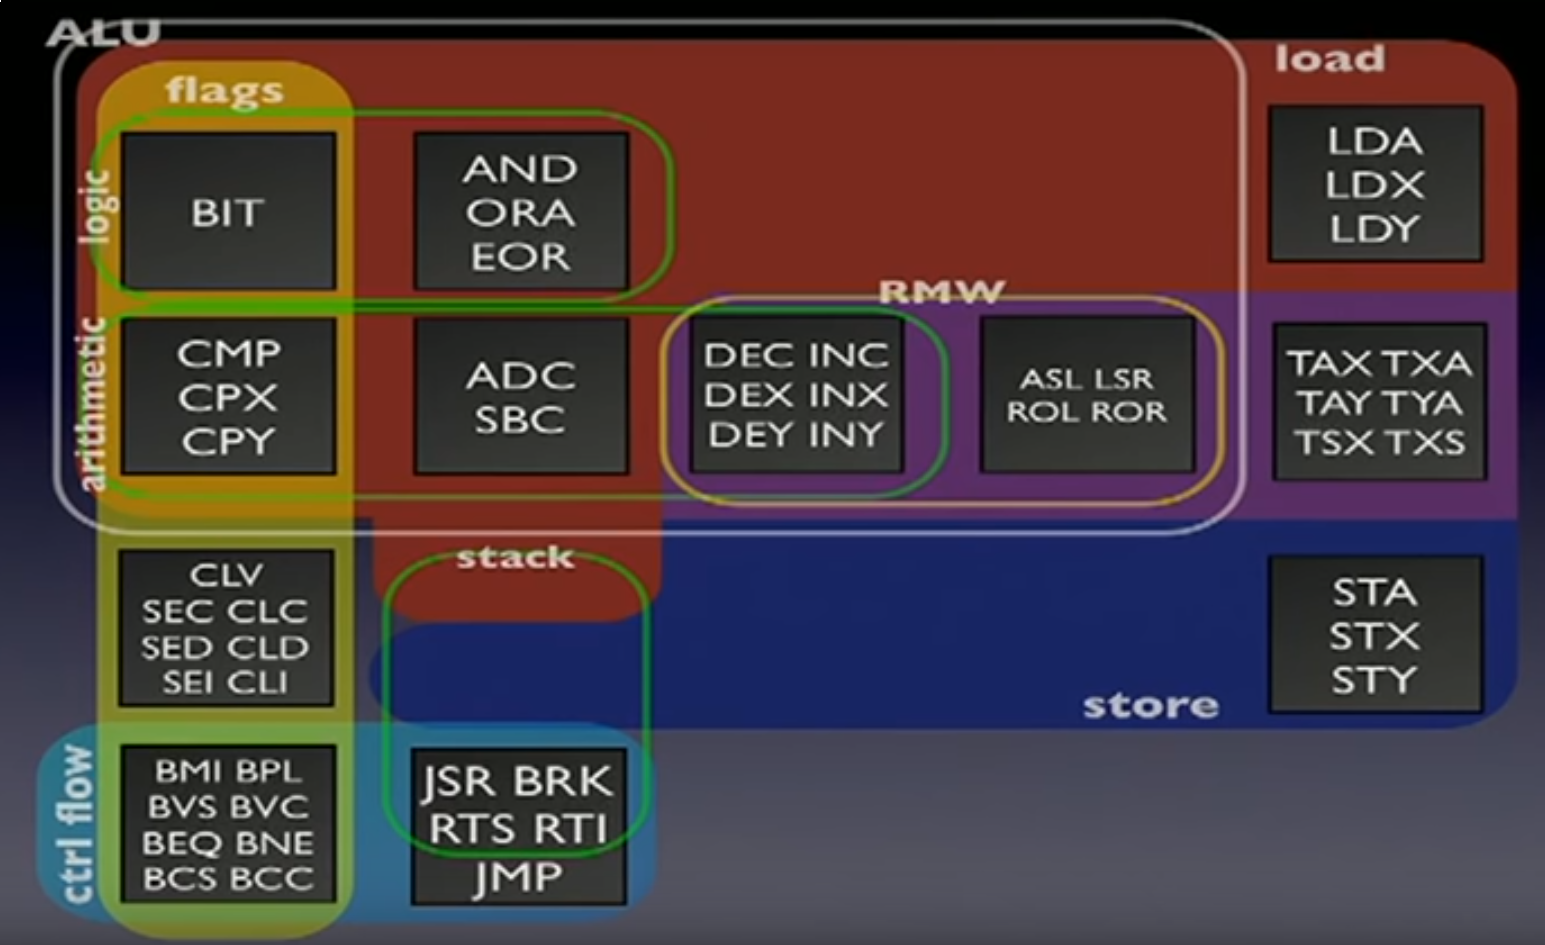
\includegraphics[width=\textwidth]
		{images/instruction_map.png}}
	\caption{\label{fig:my-label} MOS 6502 instruction map (\cite{TALK})}
\end{figure}
\clearpage


\section{RAM}

\subsection{Specification}
\paragraph{ }
The NES RAM (\cite{NSRM}), unlike RAMs nowadays, fulfils multiple purpose. One of them is providing a storage for the game program code, and the other one is to provide connection for the CPU to the other parts of the console.
\paragraph{Storage}
The console manufactured with a fix 64KB of RAM. This amount of storage was accessible trough a 16-bit address bus and a 8-bit data bus. The fact that the memory is addressed by 16-bit addresses the CPU required extra cycles to read and write from the RAM as it can only handle 8-bit values. This is where the different addressing modes for the instructions became effective useful to provide faster access to the RAM therefore increase performance.
\\
 Interestingly from the 64KB of RAM only 32KB were actually  available for the programmers to store their games' binaries. Also from this 32KB another 6 Byte comes down which are the necessary reset vectors reserved for the CPU to specify where to search for the first instruction after power-on/reset or where to jump to handle an interrupt. Other than that the developer have full access over this 32KB so called PRG ROM or Program Rom. It is separated up to two 16KB chunks as it is stored this way on the ROM Cartridges. The way how it is filled up is defined by the cartridge and it's mapper. There are tricks how to utilize more storage then 32KB but this needs a special Cartridge format, see below at section 4.3. 
 
 \paragraph{Zero page}
 On the other hand the memory has other parts which are still available for the programmer with a few restriction. Such as the Zero page. This is a special 256 Byte sized area at the very beginning of the RAM.
 As this area's address space is 0x0000 - 0x00FF to access this we only need 8-bit long address therefore the accessing speed of this part of the ram is doubled compared to the rest of it. One of the main purpose of this Zero Page area is to provide additional fast storage for the CPU to carry out complex calculations as it is already mentioned above the NES' microprocessor only contains 3 general purpose registers from which 2, the X index and Y index, has only limited capabilities for arithmetic operations.
 
 \paragraph{Stack}
 This area located right after the zero page at the address from 0x0100 up to 0x2000 reserved for the stack operations which are carried out either by a subroutine/interrupt call or forced by the programmer with the necessary CPU instructions. Interestingly, unlike on the modern systems, stack overflow never happens. Instead the stack wraps around and starts overwriting itself. Of course this behaviour contains pros and cons. For example this type of stack provides more flexibility for the developers as they can exploit this behaviour, on the other hand , it could results loss if information and crash the program as the return form interrupt or subroutine  will put the microprocessor to a wrong address therefore causing memory corruption.
 \\
 Important to notice that as the stack is reside in the RAM the developers has read and even write access to these parts of the memory. Therefore the data stored here can be manipulated without any stack specific instruction and just treating it as a normal RAM. It is dangerous but widely used at more complex games which are heavily pushing the limits set up by the hardware.
 
 \paragraph{RAM}
 The actual RAM, which in functionality identical to the modern RAMS, are 1,5KB starting from address 0x0200. This is the amount of storage space given to the developers to use it freely for their games. Technically, there is no difference between this section and the Zero Page other than the fact that the Zero page accessing time can be two times faster therefore it is better to think about it as some sort of CPU registers for performance reasons. 
 
 \paragraph{ }
 The Zero page, Stack and RAM section together mirrored three times in the upcoming 6KB to fill the addressing space up to 0x2000. Which means whenever a memory accessing carried out on the address range of 0x0800 - 0x1FFF is equivalent to do it on 0x0000 - 0x07FF.
 \\
 The reason behind this type of memory mirroring is that when the hardware decoding the given address line a lot less pins on the chip are required to do that by limiting down the address space.
 
 
 \paragraph{I/O Registers}
 The following memory addresses starting from 0x2000 up until 0x0401F are specially mapped to other parts of the NES console. This way the system provides opportunity ot the CPU, along that to the developers, to control the other hardware parts by writing or reading values from these special locations.
 \\
 0x2000 - 0x2007 address range are mapped to specific PPU, Pixel Processing Unit, Registers. Which can be used to query the current status of the PPU, control it's behaviour or even to copy data to it's VRAM. See Section 4.4 for more details.
 This range of PPU memory mappings are also mirrored through the following address place from 0x2008 up to 0x3FFF.
 \\
 In the 0x4000 - 0x401f address range the APU and Controller mappings resides. As this project not implementing the Audio Processing Unit the only important registers are the 0x4016 and 0x4017. These memory mappings provides the possibility to query the two controller's input or change it's reading behaviours.
 

\subsection{Implementation}
\paragraph{ }
The RAM implementations itself was done by using an array of 8-bit long unsigned integer pointers. Unsigned variables were used the fact, as it was mentioned above, that the CPU along with the whole system handles every value as an unsigned integer. The reason behind using an array of pointers instead of an array of values is th easily mimic the memory's mirroring behaviour. During the initialization of the RAM the same set of pointers were copied to the given parts of the array. With this when ever a given address was written every other address, the given element of the array, were updated as they all pointed to the same value.
\\
The above mentioned connections between given memory addresses and the other hardware parts was done via a listener system. Which consist an EventSource and a Listener. In this scenario the Memory is the event source and notifies all the subscribed components whenever a read or a write executed on the memory. Therefore the for instance the PPU can handle the reads and writes executed on it's mapped registers.

\subsection{Testing}
As the most part of the RAM is just reading and writing the given indexed value of the array the carried out tests were focusing on to make sure that the memory mirroring implemented properly.
\\
This was done by executing a certain sets of reads and writes to evaluate that for each write and read all the necessary memory slots were properly updated.


\begin{figure}[!htb]
	\center{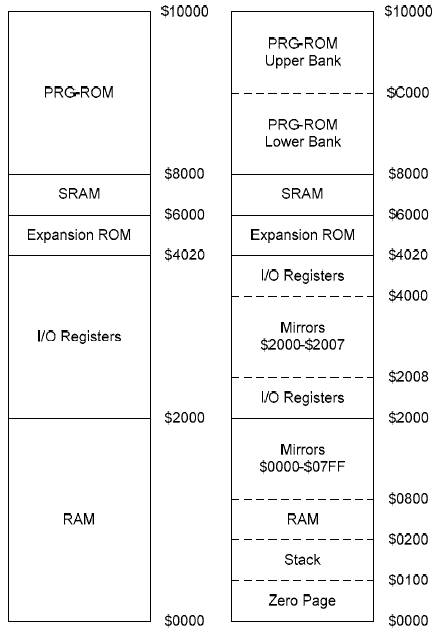
\includegraphics[width=\textwidth]
		{images/memory_map.jpg}}
	\caption{\label{fig:my-label} Memory map (\cite{NSPF})}
\end{figure}
\clearpage

\section{Cartridge (ROM)}

\subsection{Specification}
The cartridge is a very special part of the NES console ecosystem. As the hardware does not contains any storage capacity on it own, it was solved by distributing the games and the necessary programs on Cartridges. These Cartridges usually contained the program data and the sprite pattern data, for more details about the sprite data see section 4.4. Whenever one of these connected to the console then the data is loaded up from the Cartridge to the RAM and the VRAM.
\paragraph{ }
The console itself does not know where to put the data which was hold on the cartridge because they, unlike modern ROMS like DVDs and Blu-rays, came in a different layouts. To handle these differences the cartridges contains some extra special circuits called mappers (\cite{MPPR}). The mappers provides a great potential to the developers to not just deliver the necessary data of the game but to even extend the console capabilities. By design the console itself provides space for 8KB of sprite data and 32KB for program data. Just like the very first cartridges to the console, see Figure 4.3, came with an 8KB CHR ROM (sprite data) and either 16KB or 32KB PRG ROM (program codes). When the cartridge only contained 16KB of PRG ROM than the memory was filled up by copying the data twice after each other. These were the so called NROM (\cite{NROM}) mapped cartridges.
\paragraph{ }
Of course there were cartridges which designed to be more complex such us the MMC5 (\cite{MMC5})). One of the most famous game shipped with this type of Cartridge was the Castlevania III: Dracula's Curse.
The MMC5 itself was capable to ship 1MB of PRG ROM and 1MB CHR ROM which is truly extended the possibilities what a developer could achieve. But that is not everything, the cartridge also provided, along the huge storage capacity, 128KB of extra RAM for the system, extra sound channels for audio, extra interrupts on each scan-line instead of only at the VBlank. 
\\
This greatly extendable possibility through different Cartridges was one of the reason why this system was so successful and could live up until the late 90's.

\paragraph{ }
As these cartridges were designed to specially for the NES console a new file format was designed to hold a digitalized version of these cartridges. This format called iNes (\cite{INES}) or the later extended version the NES2.0 (\cite{INS2}). These formats considered by the de facto standard format for storing and distributing these old games. And also to use for emulator developers.
The usual structure of such file is the following:

\paragraph{Header section}
The first 16 byte, which from the first 3 byte is "NES<EOF>" string, is the header section. These bytes are either flags which provides some information how the console different parts meant to be configured up. Or providing details about the actual ROM file by defining what type of binary data represented within the file and what size of the given parts are.

\paragraph{Training Area}
Right after the header section, if presented, coming the training area. This is a special, fix 512 byte long sequence which used for providing extra code for compatibility reasons. This either for some special hardware inside the Cartridge or to provide helpers to run a game which was originally developed for a different gaming console but it was ported to the NES system.

\paragraph{PRG-ROM}
The upcoming part after the training area is the PRG-ROM. This section contains essentially the game logic itself. It is coming on 16KB batches and even if it is not filling up the last batch it has to be padded out to be the right size. This is required mainly for compatibility reasons, to mimic the actual PRG-ROM chip behaviour form the physical cartridges.

\paragraph{CHR-ROM}
The CHR-ROM is very similar with the PRG-ROM in behaviour within the iNes format. The difference comes form the batch sizes, as it is only 8KB rather than being 16KB. The format itself does not put restriction on the developer what they can put in here, but the mapper usually loads the data found here to the VRAM's Pattern table.

\paragraph{Miscellaneous ROM}
The remaining bytes in the file belongs to the Misc ROM. This is rarely used by special types of the console and mapper to provide some extra executable code or audio data.

\subsection{Implementation}
\paragraph{ }
The implementation of this piece of hardware was separated to two parts. First the iNes format parser and 
secondly the mapper implementation itself.
\paragraph{Parser}
Once the binary file was opend for reading purposes the first thing which has to be done is to read the first 16 byte. These bytes are the so called header of the file. The header includes important information about the cartridge. Such as how big are the PRG and CHR ROMs or is there any training area presented or which mapper meant to be used with this ROM. Once these details are carefully extracted from the header, all the necessary information available for the parser to identify what each byte represents. Knowing that, the separate portions of the file can be parsed and presented as a well structured object () which could be used by the mapper.
\paragraph{Mapper}
As there is a large pool of mappers (\cite{MPPR}) which are used in the NES system, due to time limitation and project scope only the NROM mapper was implemented.But the actual implementation was carried out in mind of the code has to be easily extendable with other mapper implementation. That leaded to the current implementation which consists an abstract Mapper class and a helper method to create a concrete mapper object based on the parsed Cartridge.

\subsection{Testing}
\paragraph{ }
The testing of the parser was implemented in a rather simple way which consisted multiple steps.
First of all a NES ROM was selected as the target of the test, due to the nature of the test it could be any valid iNes binary file. Then the selected file was parsed by the our emulator. 
\\
Based on the result of the parsing the source file was replicated then checked of the source binary file is exactly the same as the replica. 
\paragraph{ }
This theoretically supposed to be enough but as new logic introduce, namely the file replication from the parsed format, another step was required to verify it to be 100\% right. In the next step the the file which was the result of the replication was also parsed and checked if it is equal with the previously parsed object from the origin test file.  

\begin{figure}[!htb]
	\center{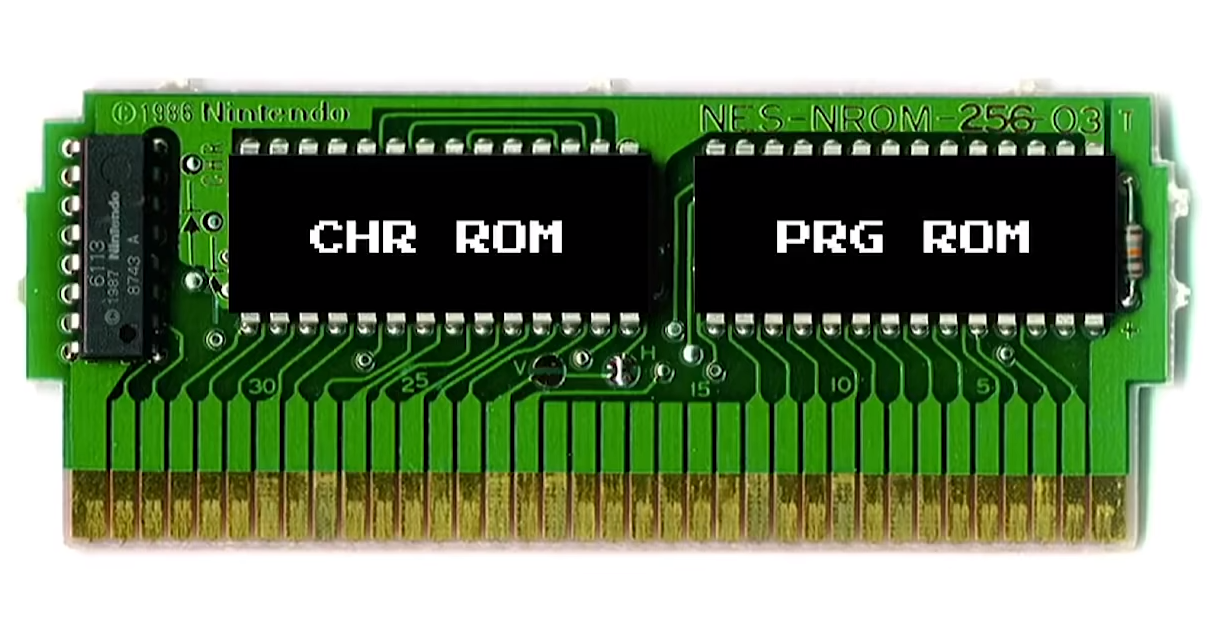
\includegraphics[width=\textwidth]
		{images/nrom_cartridge.png}}
	\caption{\label{fig:my-label} NROM cartrdige (\cite{ROM1})}
\end{figure}
\clearpage

\section{PPU}

\subsection{Specification}
\paragraph{ }
The PPU (\cite{NDPP}), Pixel Processing Unit, is one of the most complex part of the NES system, form an emulator development perspective. Compared to it's time it was a really advanced chip. Just like the CPU it was also manufactured by Ricoh and had two different version the RP2C02 and the RP2C07 for PAL regions. The chip itself contained 16KB dedicated VRam which was used to store the screen and sprite graphics. In terms of speed the PPU runs 5,36MHz, this results that meanwhile a CPU does 1 cycle the PPU executes 3 of them. And as the name show these cycles is used to draw the screen pixel by pixel with a 60FPS, Frames Per Second, based on the settings of the chip and the content of it's dedicated ram. Both of these are accessible and modifiable through memory mapped register for the CPU, therefore to the developers as well.

\paragraph{ }
The PPU contains 9 registers which are mapped to a given address of the main memory of the system. Each of these registers can be read, write or  both to control the behaviour of the PPU (\cite{PPRG}). Whenever any of these accessing happens it goes through a special latch. This latch is capable to hold data temporarily when ever a read or a write happens. It is most useful when larger 16-bit numbers are transferred between the CPU and the PPU as both chip handles only 8-bit values.

\paragraph{PPUCTRL}
This register mapped to the main memory at 0x2000. It can be used by writing an 8-bit value to the address where  each bits has it's own effect on the PPU.
\\
Bit 0 and 1 can be used to select which nametable out of the four meant to be the main one.
\\
Bit 2 sets elopment perspective. Compared to it's time it was a really advanced chip. Just like the CPU it was also manufactured by Ricoh and had two different version the RP2C02 and the RP2C07 for PAL regions. The chip itself contained 16KB dedicated VRam which was used to store the screen and sprite graphics. In terms of speed the PPU runs 5,36MHz, this results that meanwhile a CPU does 1 cycle the PPU executes 3 of them. And as the name show these cycles is used to draw the screen pixel by pixel based on the settings of the chip and the content of it's dedicated ram. Both of these are accessible and modifiable through memory mapped register for the CPU, therefore to the developers as well.

\paragraph{ }how the memory address pointer incremented after each data writing. This is mostly used for nametables, as it is provided an option to fill them line by line or column by column.
\\
Bit 3 provided an option to select which pattern table used to supply the graphics details for sprite rendering.
\\
Bit 4's behaviour is the same as bit 3's, the difference is that this bit set the source palett table for the background evaluation.
\\
Bit 5 was the flag which used to toggle between 8x8 and 8x16 sprite size.
\\
Bit 6 is meant to be used to change the behovior of the EXT pin on the PPU chip but due to tits formation when it set it can damage the board therefore its highly discouraged to set this flag.
\\
Bit 7 is the NMI flag. When this flag is set and the PPU reaches the VBlank state it generates an NMI interrupt in the CPU.

\paragraph{PPUMASK}
The register which is mapped to the 0x2001 memory address is responsible for masking options. The register is write-only. With these writes the way how the PPU colors the pixels can be changed.
\\
Bit 0 is used to toggle greyscale colour rendering.
\\
Bit 1 can be used to toggle the rendering of the background for the first column of the screen (8 pixel on the left side of the screen).
\\
Bit 2 identical with bit 1 except it used for the sprites.
\\
Bit 3 is the flag which toggle when ever the background should be rendered or not.
\\
Bit 4 is again identical with bit 3 but it toggles the sprite rendering.
\\
Bit 5, 6 and 7 used to make the Red, Green and Blue colour  displayed stronger.

\paragraph{PPUSTATUS}
This is a read only register, at memory location 0x2002, used to report back events which generated meanwhile the screen is rendered. Also reading this register has a side effect on the above mentioned latch which is used for communication between the CPU and the PPU and also on itself. Namely after every read Bit 7 became 0 and the address latch is set back to the default nametable address which is set by the control flag.
\\
Bit 5 is set when in a single scanline more than eight sprite meant to be rendered.
\\
Bit 6 is set when any of the non transparent part of a rendered sprite overlaps with a non transparent part of the background.
\\
Bit 7 is set when the PPU reached the VBlank state.

\paragraph{OAMADDR}
This write-only register used to specify the OAM, Object Attribute Memory, address. This address fulfils multiple purpose. One is to provide and address which specify the data which should be red or overwritten by the OAMDATA registers. The other is to set which byte is the first byte used in the OAM ram when the sprites are rendered on the screen. This register is mapped to 0x2003.

\paragraph{OAMDATA}
This register used to either retrieve data or set it in the OAM memory. Both of these functionality can be achieved with the corresponding read or write to the 0x2004 memory location. To carry out both functionality the OAMADDR register's value used as an address. Important to notice as this register modifies the sprite data it is highly discouraged to write to it meanwhile the screen is under rendering to prevent rendering errors.

\paragraph{OAMDMA}
OAMDMA register is used to trigger a DMA, Direct Memory Access, by writing an 8-bit value to the 0x4016 memory address. This 8 bit value will be used than as the high byte for accessing the memory and filling up the OAM memory by coping the values from 0x\#\#00 - 0x\#\#FF memory location where the \#\# is the 8-bit value above mentioned. Meanwhile DMA is carried out by the PPU, the both the data and address bus of the main memory is occupied therefore the CPU is unable to fetch the next instruction and carry on until the DMA is not finished. Due to this and the fact that the PPU works 3 times faster than the CPU this is the preferred way to populate the OAM memory due to performance reasons.

\paragraph{PPUSCROLL}
PPUSCROLL register used to modify the background rendering starting point, which is set by the PPUCONTROL register, by adding a certain offset to it. This offset can be specified by two writing to this register at memory location 0x2005. At the first write the X offset will be set and on the second write the Y offset will be set. It is highly recommended to execute a PPUSTATUS read before this operation to make sure the base address is pointing to the right place and no garbage value left behind by any previous operations.

\paragraph{PPUADDR}
To set the value of this register two writes necessary to the 0x2006 address, as the VRam, just like the main memory, working with 16-bit addresses. Important to notice that the first the upper 8-bit, and with the second writing the lower 8-bit can be set.

\paragraph{PPUDATA}
Right after the PPUADDR at 0x2007 this register responsible to writing data or return the data from the VRam address specified by the previously mentioned register. After each write/read the PPUADDR register will be incremented based on the settings specified in the PPUCONTROL. Along with the address increment there is another hidden behaviour. Every read for this register is buffered, which means to read the right value after changing the address register two reads has to be performed and with the second read the right value will be returned.

\paragraph{ } 
The PPU's own dedicated VRam. Even though the 16-bit addressing let the system address up to 64KB,  in reality it only uses 16KB due to cost efficiency in my when the hardware was assembled.
Therefore each access which targets address 0x4000 or above will be mapped down to an appropriate address.
\\
The VRam is separated up to multiple section. Each of these combined together producing the screen which is displayed on the television screen.

\paragraph{Pattern Table} 
The pattern table \cite{PTRN} is a 4KB section inside the VRam. It is occupying the 0x0000 - 0x0FFF and 0x1000 - 0x1FFF address space as there is two of them.  These pattern tables is used to store sprite patterns.  Each of these sprite patterns describes an 8x8 pixel blocks. A sprite pattern consist of 16 Bytes which used to describe which colour meant to be used to draw each of the pixels within this block. The colours used by the PPU to draw these pixels are aligned in colour . Each of these pallets contained 3 different colours and background colour, therefore 2 bits was required for each pixel to identify which colour needed to be used. That is why the 16 Byte was utilized in a certain way. The first 8 byte sets the low bit of the colour by storing each 8 wide line information as a byte from top to bottom. The second 8 byte works in a similar fashion but it provides high bit of the colour.
\\
The above described structure also well represented in the actual addressing as well. Whenever a byte in the pattern table addressed the top 4 bit sets which pattern table are meant to be used it could be ether 1 or 0. The next 8 bit used to identify which pattern are targeted. Meanwhile the least significant 4 bit of the address used to identify the number of the pixel rows, 0x0 - 0x7 low bit rows, 0x8 - 0xF high bit rows.

\paragraph{Name Table}
The name table (\cite{NMTB}) is the part of the VRam where the background is stored. One of the name tables hold enough information to cover the whole screen. To do this, a single name table is 960 bytes long which is enough to fill the while screen with 8x8 pixel blocks, where each block is represented by a single byte. The byte was needed to store the pattern index for colouring the block. Inside the memory the name table bytes are aligned by row by row starting with the byte of the top leftmost 8x8 pixel block. Although to provide scrolling functionality more than one was needed. 
\\
The PPU designed to be able to handle four of them to provide proper vertical and horizontal scrolling functionality at the same time. To do this the PPU used the four name table as they are ordered in a 2x2 manner and a 1x1 name table sized portion was selected from this to be drawn on the screen.
The four name table can be found in the memory each starting at the given addresses: 0x2000, 0x2400, 0x2800, 0x2C00.
\\
 But as the system was not shipped enough VRam just for two name table the other two were just mirrors. The way how the mirroring executed is specified by the cartridges. There is two way how the PPU on its own can implement the mirroring. Either vertical, when the top 2x1 name table is equals the bottom 2x1 name table or horizontal, when the left 1x2 name table are mirrored to the right 1x2 name table section. In these cases background scrolling only works in one direction.
 \\
On the other hand, games like the Super Mario Brothers 3 implements scrolling on both direction at the same time. This was achieved by shipping extra ram for the PPU inside the Cartridge. These extra ram then used to provide enough space to use 4 different name table at the same time.


\paragraph{Attribute Table}
Right after each name table in the memory there is a 64 byte long attribute table (\cite{ATRT}). This section of the memory hold data that provides information about which colour palette used for each 8x8 pixel block described in the name table. As the size of this section not enough to cover each name table entry one by one, a more compressed structure is used.
\\
Each 8-bit entry, that contains 4 different 2-bit long pattern table index, refers to a 4x4 block of name table entries. The 4 index is divided up between the included pixel blocks by following the convention that the least significant 2 bit refers to the top-left 2x2 block, within the 4x4 target, the next 2 bit specifies the top-right section, the 4th and 5th bit belongs to the bottom-left one and the 2 most significant bit describes the bottom-right 2x2 name table entry block.
\\
Although, this solution is storage efficient it comes with certain drawbacks. Mainly it reduces how many colours can be displayed on the background per frame as each colour colour palette is referenced by multiple adjacent nameable entry. Also due to this grouping, when screen-scrolling involved the side of the screen can suffer from colour glitch, this can especially noticed at the right side of the screen while playing Super Mario Brothers 3.

\paragraph{Palette Table}
Lacikam

\paragraph{ }
Along this there is a separate 256 Byte area called OAM, Object Attribute Memory, where the sprites attributes are stored. This provides enough storage for 64 different sprite as each sprite attribute is 4 byte. 
\\
The 1st byte and the 4th byte specifies the Y and the X coordinate of the sprite on the screen. The 2nd byte gives the index of which patten meant to be used to render the given sprite. Closely related to that the 3rd byte provides some flags which can change the behaviour of the rendering for the specific sprite only. 
\\
With the bit 0 and 1 the colour palette for the sprite can be set. Bit 7 and 6 provides capability to draw the sprite vertically and/or horizontally flipped, this is a very usefully capability of the PPU which could save up a huge amount of palette RAM. For example the big mario character instead of using 6 different pattern it can be made using only 3. by using a flipped version of the chest and leg part.
\\
 Also, with bit 5 we can set the rendering priority of the sprite. Which could result that the sprite will be rendered behind non-transparent background elements.
 
 \begin{figure}[!htb]
 	\center{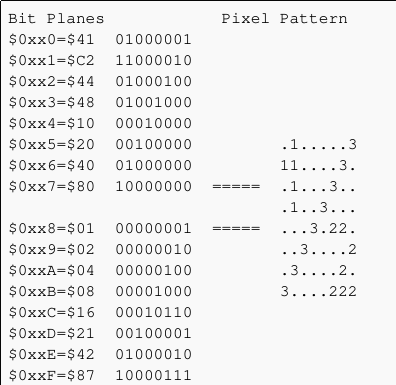
\includegraphics[width=\textwidth]
 		{images/pattern_example.png}}
 	\caption{\label{fig:my-label} Pattern table example (\cite{PTRN})}
 \end{figure}
 \clearpage

\subsection{Implementation}

\subsection{Testing}

 \chapter{Evaluation}

\section{Performance and Precision}

\section{Game Performance}

\chapter{Conclusions}

\printbibliography

\end{document}          